% Created 2020-10-12 Mon 10:58
% Intended LaTeX compiler: pdflatex
\documentclass[presentation]{beamer}
\usepackage[utf8]{inputenc}
\usepackage[T1]{fontenc}
\usepackage{graphicx}
\usepackage{grffile}
\usepackage{longtable}
\usepackage{wrapfig}
\usepackage{rotating}
\usepackage[normalem]{ulem}
\usepackage{amsmath}
\usepackage{textcomp}
\usepackage{amssymb}
\usepackage{capt-of}
\usepackage{hyperref}
\usetheme{UoB}
\author{Mark Blyth}
\date{\textit{[2020-10-12 Mon]}}
\title{Investigating spline numerics}
\hypersetup{
 pdfauthor={Mark Blyth},
 pdftitle={Investigating spline numerics},
 pdfkeywords={},
 pdfsubject={},
 pdfcreator={Emacs 27.1 (Org mode 9.3)}, 
 pdflang={English}}
\begin{document}

\maketitle

\section{Background}
\label{sec:org52536e7}
\begin{frame}[label={sec:orgb754af8}]{Week's goals}
\begin{itemize}
\item Fix splines CBC code
\begin{itemize}
\item Done for the non-adaptive case
\end{itemize}
\end{itemize}
\vfill
\begin{itemize}
\item Investigate whether the code now works
\begin{itemize}
\item It doesn't
\end{itemize}
\end{itemize}
\vfill
\begin{itemize}
\item Writing (continuation paper, extended conference paper)
\begin{itemize}
\item Happening slowly
\end{itemize}
\end{itemize}
\end{frame}

\section{CBC code}
\label{sec:org77c3cf6}
\begin{frame}[<+->][label={sec:org62e38d6}]{CBC code issues}
\begin{enumerate}
\item Results displayed incorrectly
\begin{itemize}
\item Duffing output amplitude was being calculated incorrectly
\item Fixed now!
\end{itemize}
\item Exterior knot computation was hacky
\begin{itemize}
\item Exterior knots are necessary to fit data at endpoints; I was letting SciPy recalculate them each time
\item Implemented my own exterior knot calculation method
\item Issue: SciPy gives different results when used in different ways; most robust method seems to combine my exterior knots and SciPy exterior knots
\end{itemize}
\item Adaptive knots might not be used correctly
\begin{itemize}
\item Definitely were correct in the original script
\item Might not be in the rewrite
\item Haven't checked this; avoiding the adaptive knots method for now
\end{itemize}
\end{enumerate}
\end{frame}

\section{Plots}
\label{sec:org958de54}
\begin{frame}[label={sec:org411d584}]{Fixed plotting}
\begin{center}
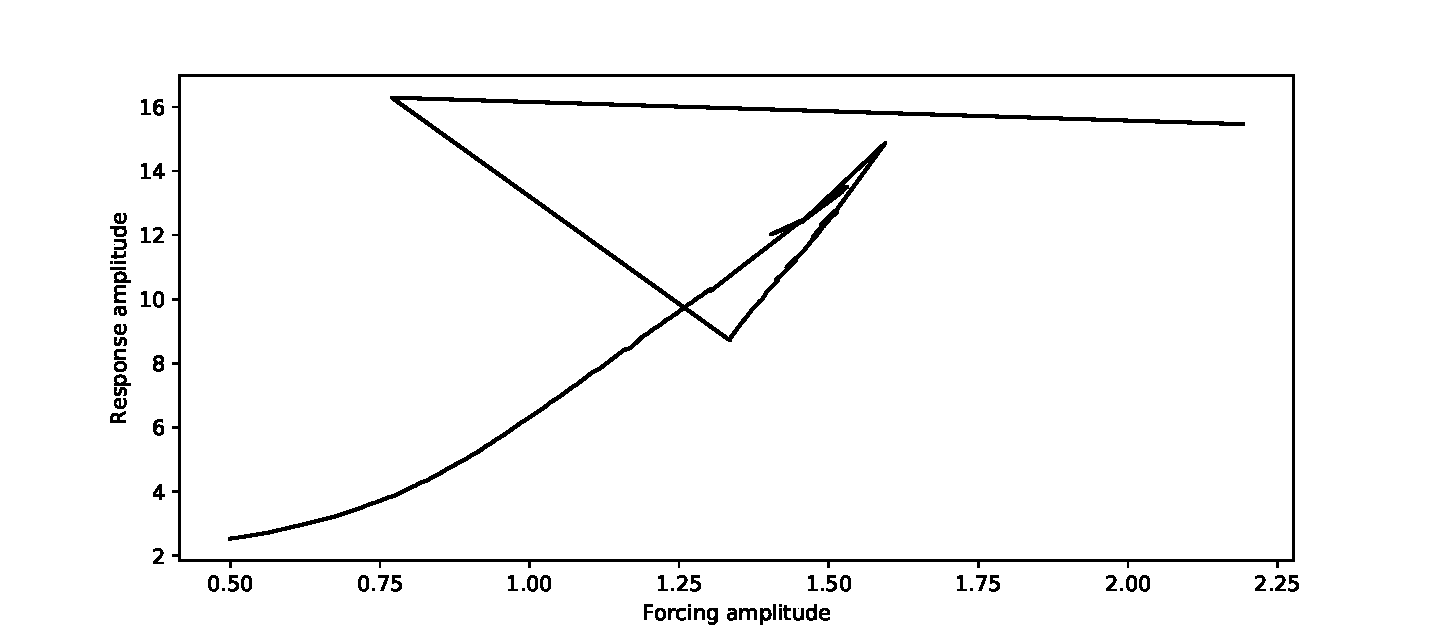
\includegraphics[width=.9\linewidth]{./stepsize0d1_dsize3_fdss0d2_fixed_plotting.pdf}
\end{center}

Stepsize 0.1; 3 interior knots; FDSS 0.2
\end{frame}

\begin{frame}[label={sec:orgff1e6b2}]{Fixed plotting: zoomed in}
\begin{center}
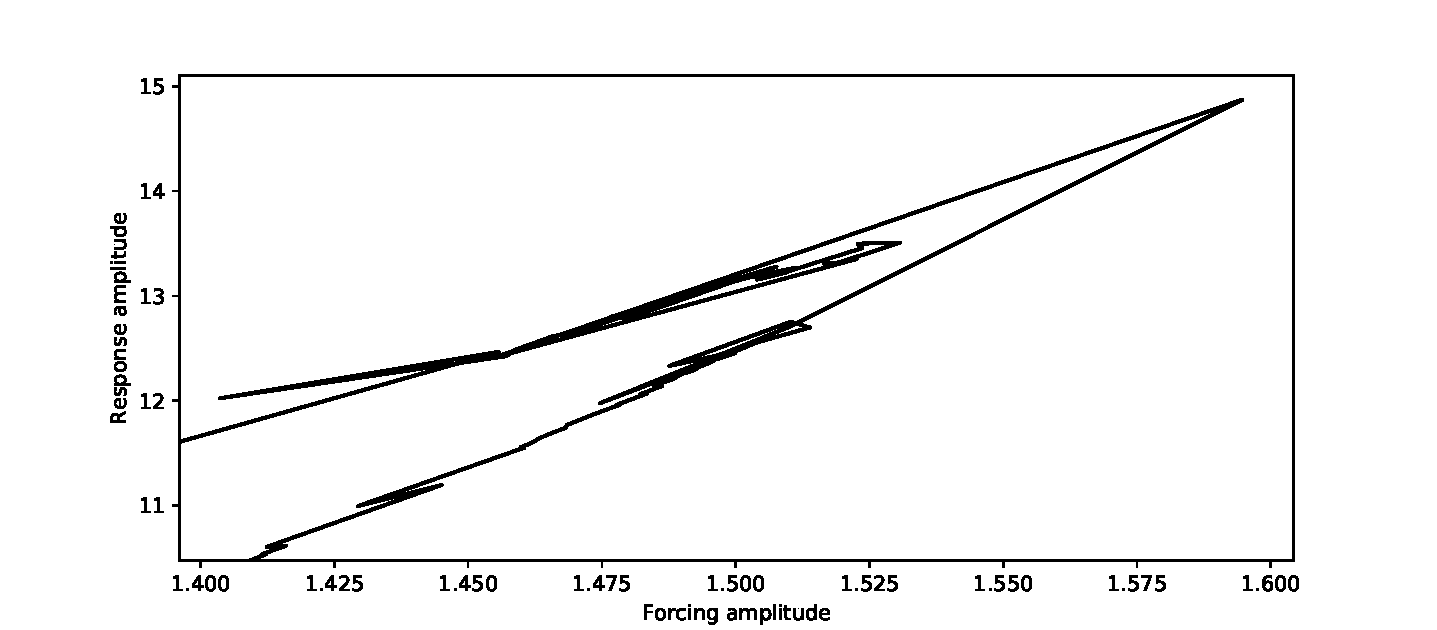
\includegraphics[width=.9\linewidth]{./stepsize0d1_dsize3_fdss0d2_fixed_plotting_ZOOM.pdf}
\end{center}

Bigger stepsize?
\end{frame}

\begin{frame}[label={sec:org9160a5c}]{Fixed plotting, bigger steps}
\begin{center}
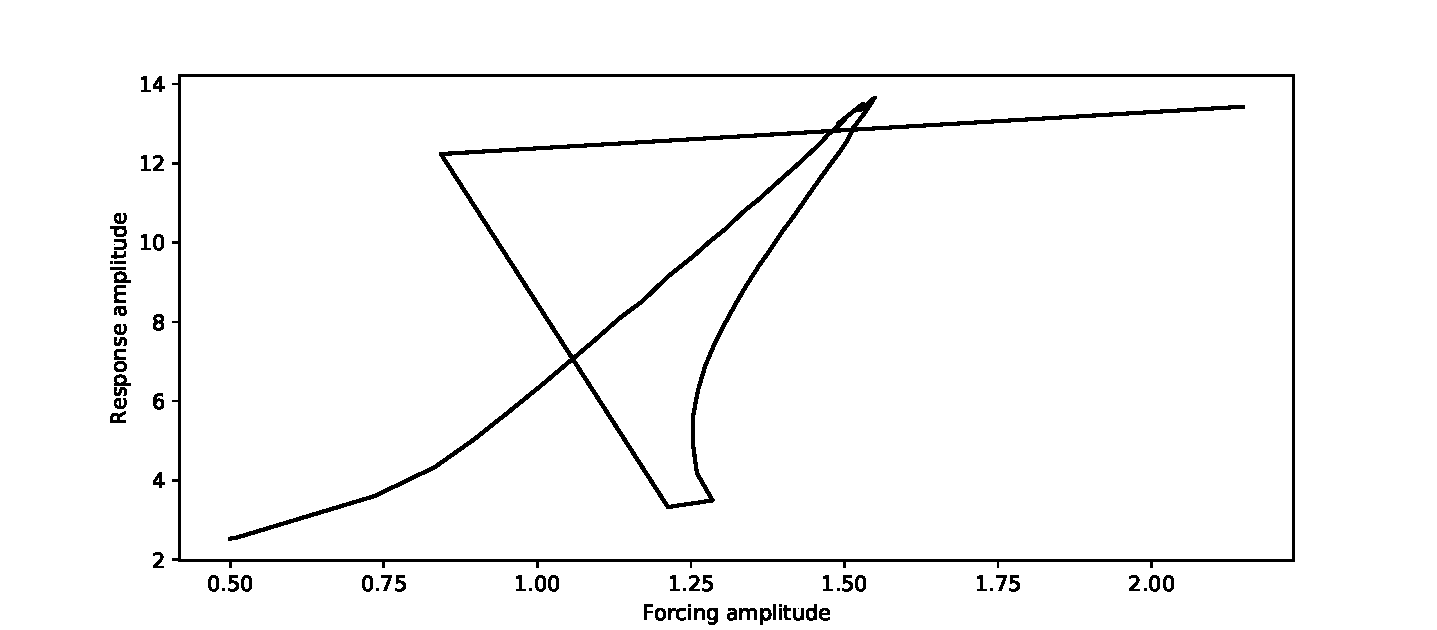
\includegraphics[width=.9\linewidth]{./stepsize1_dsize3_fdss_0d2_fixed_plotting.pdf}
\end{center}

Stepsize 1; 3 interior knots; FDSS 0.2; better, but solution jumps; let's change exterior knots
\end{frame}

\begin{frame}[label={sec:org9bb7029}]{New exterior knots}
\begin{center}
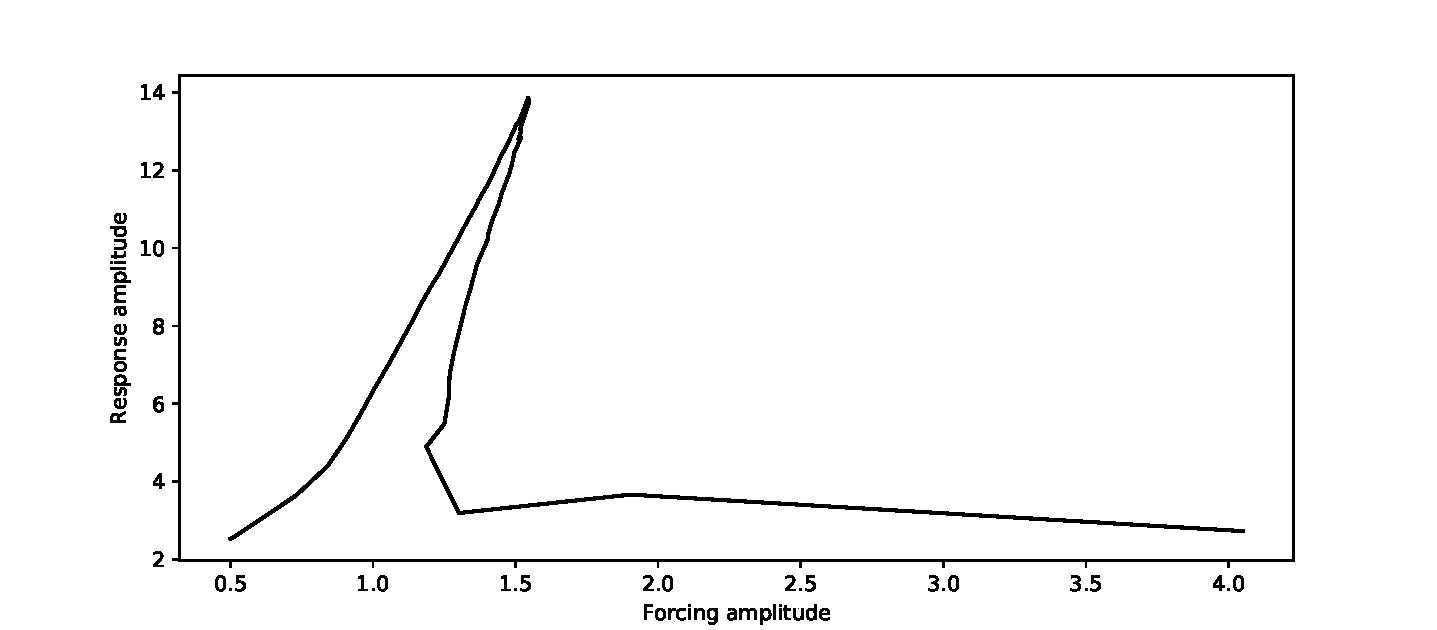
\includegraphics[width=.9\linewidth]{./stepsize1_dsize3_fdss_0d5_fixed_plotting_new_exterior_knots.pdf}
\end{center}

Stepsize 1; 3 interior knots; FDSS 0.5; fixed exterior knots; \alert{converged vectors are often not actually solutions}
\end{frame}

\begin{frame}[label={sec:orgbd896b5}]{New convergence criteria}
\begin{center}
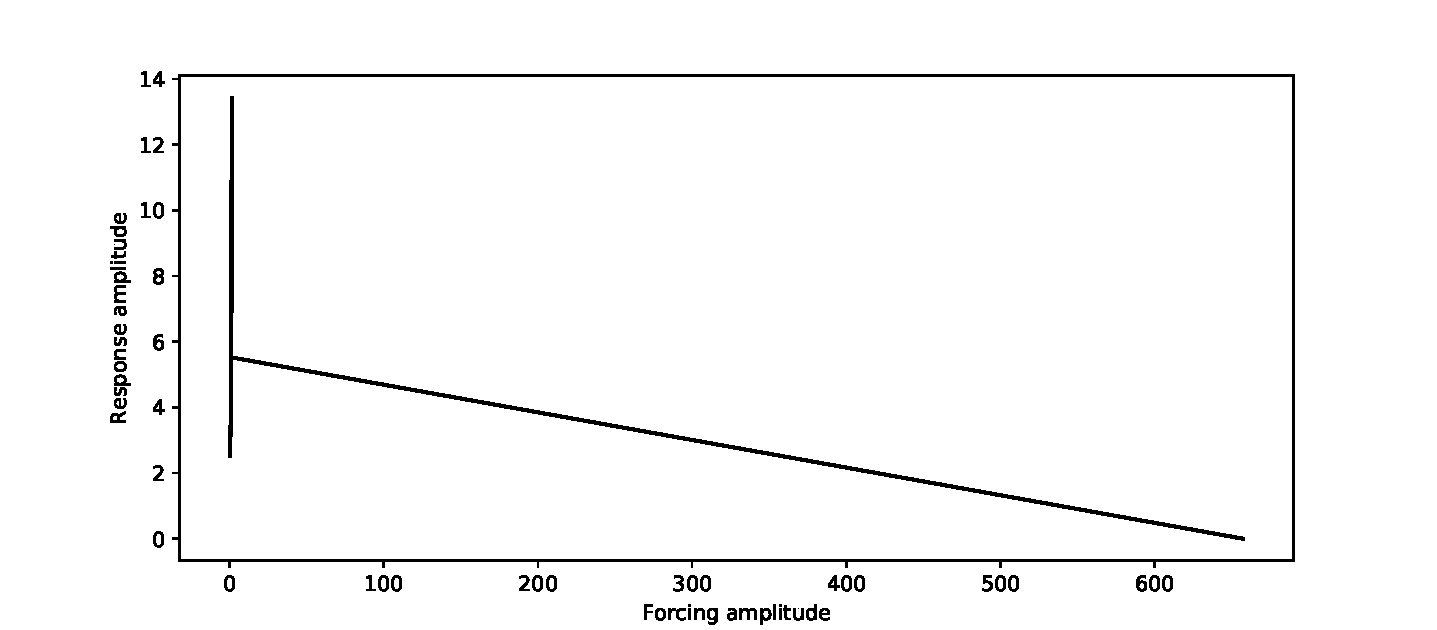
\includegraphics[width=.9\linewidth]{./stepsize1_dsize3_fdss_0d5_fixed_plotting_new_exterior_knots_5e-2solution_norm.pdf}
\end{center}

Same hyperparameters as before; convergence declared when continuation equation output has a norm below 5e-2
\end{frame}


\begin{frame}[label={sec:org9307a19}]{New convergence criteria}
\begin{center}
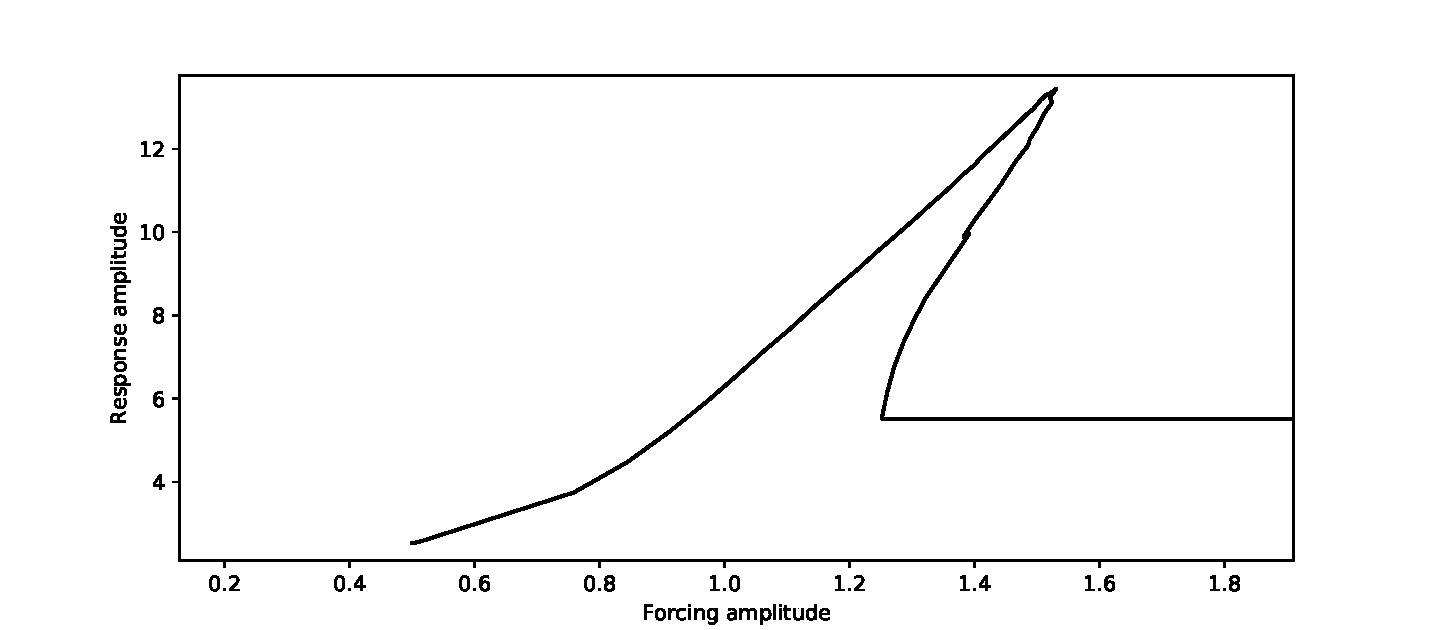
\includegraphics[width=.9\linewidth]{./stepsize1_dsize3_fdss_0d5_fixed_plotting_new_exterior_knots_5e-2solution_norm_ZOOM.pdf}
\end{center}

Zoom in to before the jump; more knots might make the results better
\end{frame}

\begin{frame}[label={sec:org6c6c3e5}]{Old convergence criteria, but more knots}
\begin{center}
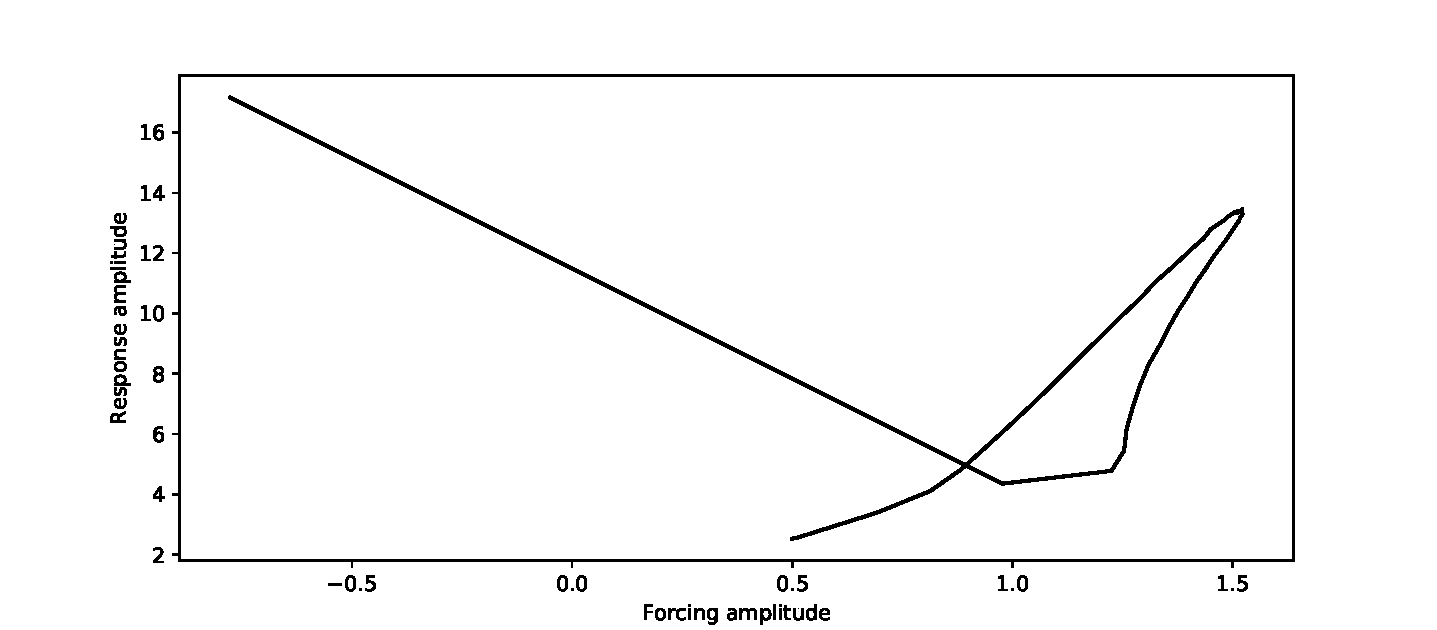
\includegraphics[width=.9\linewidth]{./stepsize1_dsize8_fdss0d5_fixed_plotting_new_exterior_knots.pdf}
\end{center}

Stepsize 1; 8 interior knots; FDSS 0.5; solution still jumps!
\end{frame}

\begin{frame}[label={sec:org22a292f}]{Best I could get}
\begin{center}
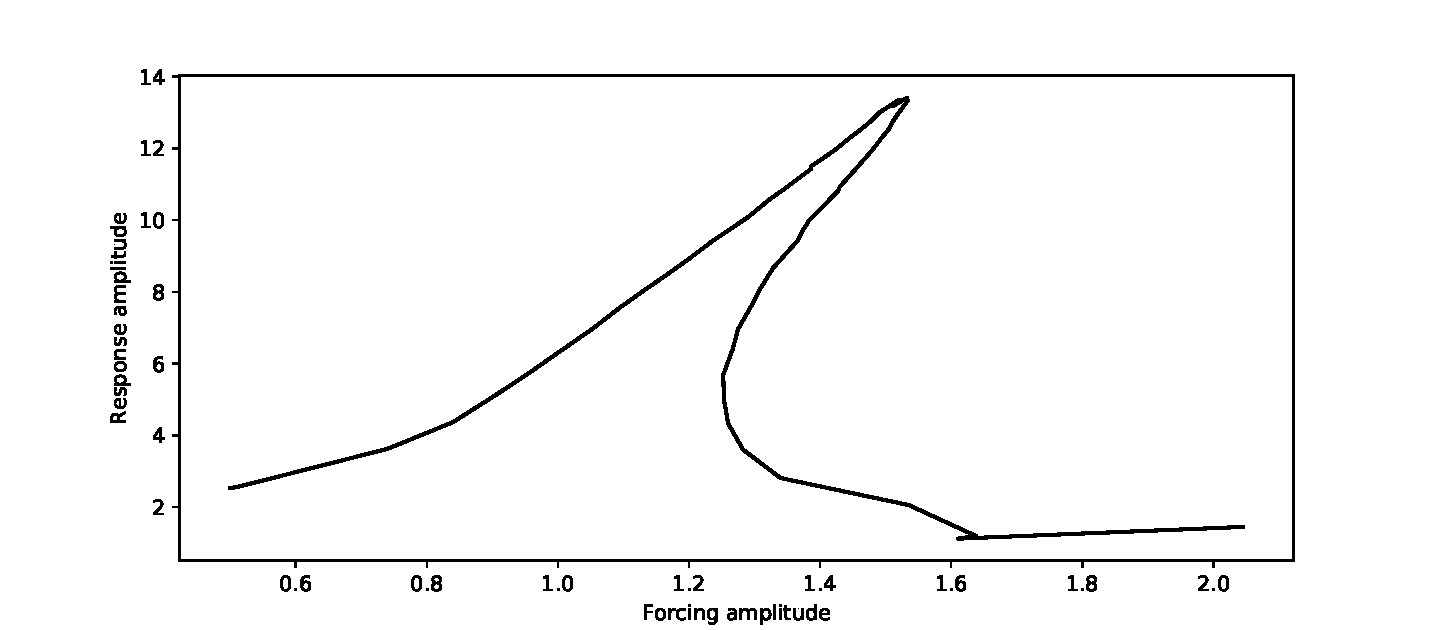
\includegraphics[width=.9\linewidth]{./stepsize1_dsize3_fdss_0d2_fixed_plotting_new_exterior_knots.pdf}
\end{center}

`Simple' convergence criteria; stepsize 1; 3 interior knots; FDSS 0.2
\end{frame}

\section{Issues}
\label{sec:orga4ca128}
\begin{frame}[label={sec:orgf2662e7}]{Issues}
\begin{itemize}
\item Hyperparameters are very hard to select
\begin{itemize}
\item Lots of trial and error to get even remotely close to the real results
\end{itemize}
\end{itemize}
\vfill
\begin{itemize}
\item Solution usually jumps near the second fold
\begin{itemize}
\item Pseudo-arclength condition is met, so the equations are fine
\item Solution is often not actually a solution!
\item Either the solver is broken, or the full system is misbehaving
\end{itemize}
\end{itemize}
\end{frame}

\begin{frame}[label={sec:org14f099c}]{Non-solutions}
\begin{itemize}
\item We're solving for \(F(x_\omega) = 0\)
\begin{itemize}
\item Newton iterations: declare convergence when \(\|x^i_\omega - x^{i-1}_\omega\| < tol\)
\item Issue: converged \(x_\omega\) typically does not solve \(F(x_\omega)=0\)
\item Alternative: converge when \(\|F(x_\omega)\| < tol\)
\item Even for \(tol\in\mathcal{O}(10^{-3})\), we never converge
\item Solution vector components jump around, rather than converging; unexpected for Newton solvers
\end{itemize}
\end{itemize}
\vfill
\begin{itemize}
\item Either solver is problematic, or equations are
\begin{itemize}
\item Using a Newton solver; simple code, tried and tested in the Fourier case
\item Finite differences are meaningful: \(\mathcal{O}(0.1)\) perturbations to \(\mathcal{O}(1)\) coefficients
\item If the solver and equations are correct, perhaps the equations are simply unsuitable?
\end{itemize}
\end{itemize}
\end{frame}

\begin{frame}[label={sec:orga21762a}]{Existence and uniqueness}
Does a solution to \(F(x_\omega)=0\) actually exist?
\begin{itemize}
\item Continuous case:
\begin{itemize}
\item A natural periodic orbit of the system exists
\item This natural periodic orbit necessarily gives noninvasive control
\item Noninvasive control means \(F(x_\omega) = 0\), so solutions must exist
\end{itemize}
\item Discretised case:
\begin{itemize}
\item We can exactly represent the continuous problem as an infinite-dimensional Fourier problem
\item As the continuous solution exists, so too must the infinite-dimensional discretised problem
\item Due to how the Fourier errors decay, we can be sure that finite-dimensional Fourier discretisation produces a solvable continuation system
\item \alert{We don't get this guarantee with splines}
\end{itemize}
\end{itemize}
\end{frame}

\begin{frame}[label={sec:org8cfbd45}]{Approximate solutions}
Does a splines solution exist? When? Thought experiment:
\begin{itemize}
\item Run the system uncontrolled
\item Discretise the output
\item Use the discretised output as a control target
\end{itemize}
\vfill
Imperfect discretisation: control target \(\neq\) `natural' oscillations
\begin{itemize}
\item Control becomes invasive
\item Control target is not a solution to the continuation equations 
\begin{itemize}
\item Even though it was obtained from an exact solution, it is not actually a solution; discretisation error stops the natural system behaviour from being a solution
\end{itemize}
\end{itemize}
\vfill
\alert{Discretisation error must be negligable for the standard CBC zero problem to become solvable}
\end{frame}

\begin{frame}[label={sec:org2388164}]{Key result}
\begin{itemize}
\item If we have no discretisation error, solution exists to continuation equations
\end{itemize}
\vfill
\begin{itemize}
\item If we have discretisation error, solution might not exist
\end{itemize}
\vfill
\begin{itemize}
\item This explains why Fourier works, splines don't
\begin{itemize}
\item No discretisation error for infinite Fourier
\item Can achieve negligable discretisation error for truncated Fourier
\item Harder to remove spline discretisation error
\end{itemize}
\end{itemize}
\vfill
How accurate are splines?
\end{frame}

\begin{frame}[label={sec:org561a04d}]{Spline discretisation error}
\begin{center}
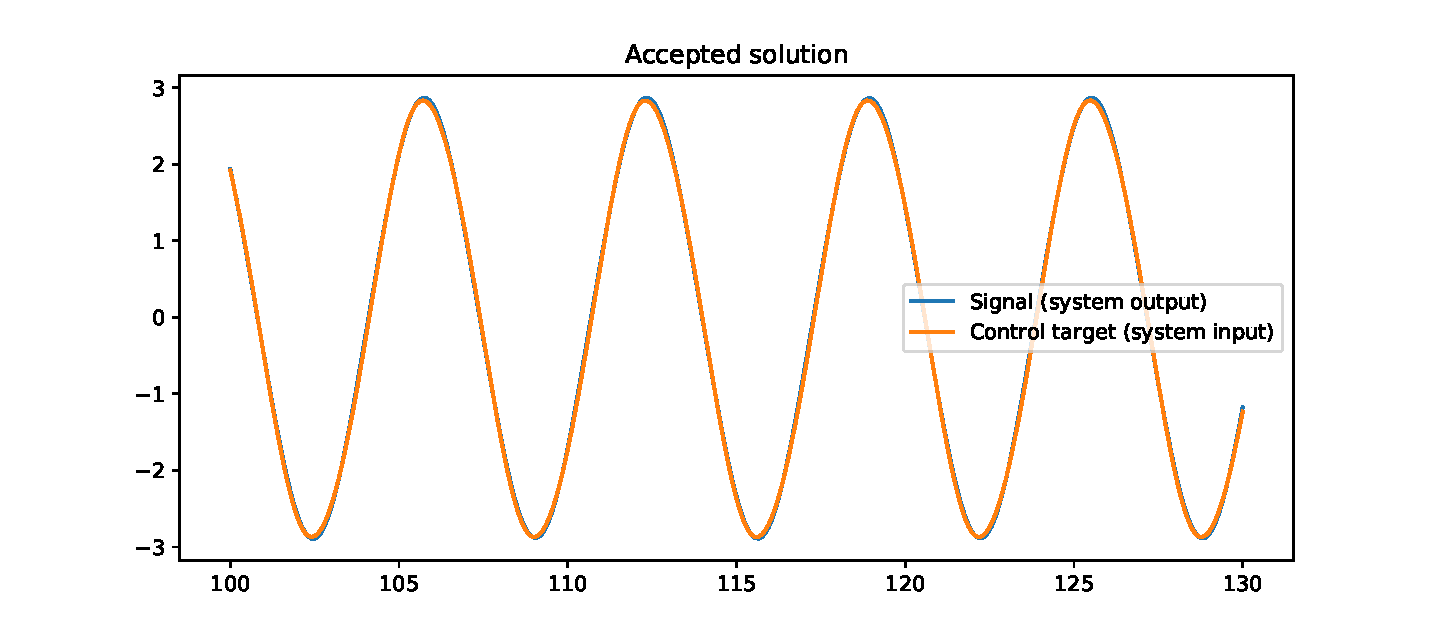
\includegraphics[width=.9\linewidth]{./good_solution.pdf}
\end{center}   

Splines is often very accurate
\end{frame}

\begin{frame}[label={sec:orgff52521}]{Spline discretisation error}
\begin{center}
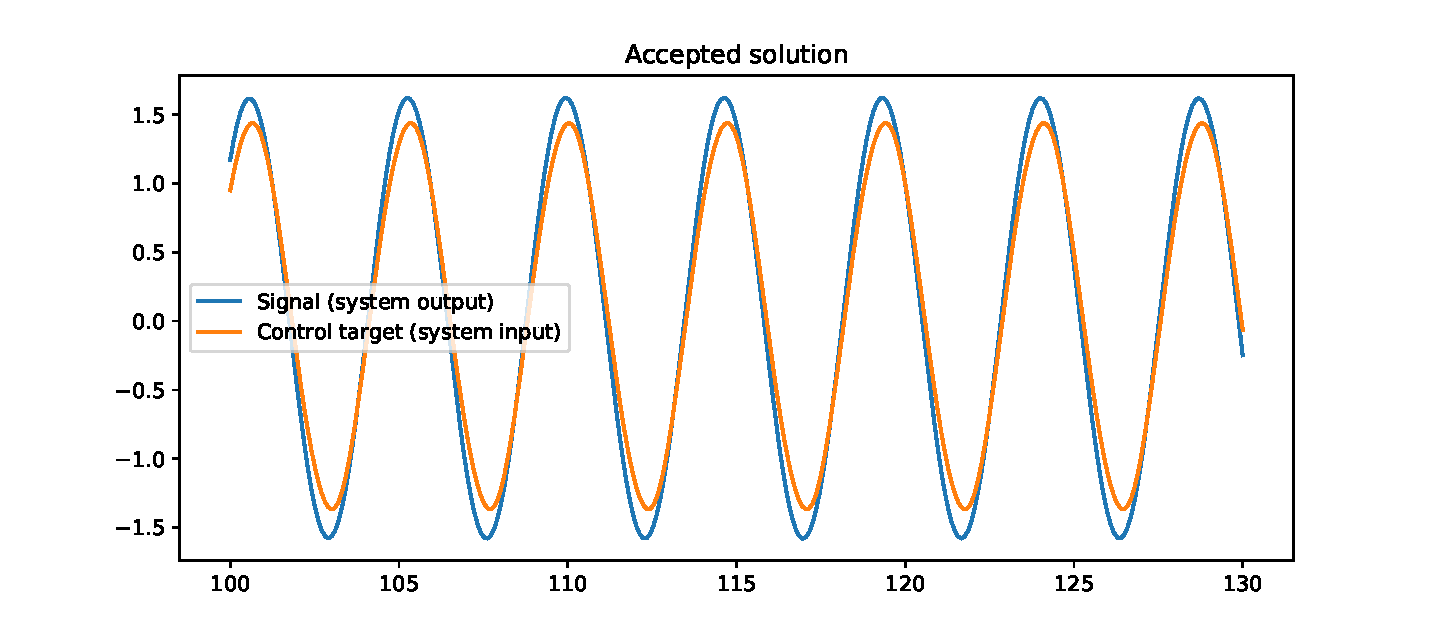
\includegraphics[width=.9\linewidth]{./bad_solution.pdf}
\end{center}

But sometimes not
\end{frame}


\begin{frame}[label={sec:orgf862f51}]{Minimization reformulation}
\begin{itemize}
\item A solution is not guaranteed to exist when the spline fit isn't exact
\end{itemize}
\vfill
\begin{itemize}
\item We can fix this with new, more general continuation equations
\end{itemize}
\vfill
\begin{itemize}
\item Solve for least invasive control target, instead of noninvasive control
\begin{itemize}
\item Solution will be noninvasive (same solution as for standard continuation equations) when discretisation is exact
\item Solution is still guaranteed to exist when discretisation is inexact
\item Solution is noise-robust
\end{itemize}
\end{itemize}
\end{frame}


\begin{frame}[label={sec:org244ff5d}]{Minimization reformulation}
\begin{itemize}
\item Let \(\beta\) be the discretisation
\end{itemize}
\vfill
\begin{itemize}
\item Let \(\mathrm{invasiveness}(\beta) = \int \left[ \mathrm{signal}(t)-\mathrm{target}(\beta, t)\right]^2\mathrm{d}t\)
\begin{itemize}
\item Valid for proportional control
\item Can be easily adapted for other control strategies
\end{itemize}
\end{itemize}
\vfill
\begin{itemize}
\item Continuation equations:
\begin{itemize}
\item \(\frac{\partial \mathrm{invasiveness}}{\partial \beta_i} = 0\)
\item predictor \(\perp\) corrector
\item This can be solved using numerical integration and standard Newton iterations; \alert{no need for minimization}: no experimental Hessians needed
\item Alternatively, solve using EGO minimizers; no experimental Jacobians needed
\end{itemize}
\end{itemize}
\end{frame}



\section{Next steps}
\label{sec:orgf47ae11}
\begin{frame}[label={sec:orgd1b1634}]{Next steps}
\begin{itemize}
\item Write splines without SciPy
\end{itemize}
\vfill
\begin{itemize}
\item Try minimizer approach; possibly slower; will guarantee finding an acceptable solution
\end{itemize}
\vfill
\begin{itemize}
\item Try adaptive-knots BSplines
\begin{itemize}
\item In general, optimization-based knot choice will minimize the discretisation error
\item Duffing is simple enough that adaptive knots shouldn't change the results much
\end{itemize}
\end{itemize}
\vfill
\begin{itemize}
\item Talk to Krasi about approximation and existence of continuation solutions
\end{itemize}
\vfill
Also, writing, annual review
\end{frame}
\end{document}
